\documentclass[11pt,oneside]{report}
\usepackage[margin=1in]{geometry}
\usepackage{amsmath,amssymb,booktabs,tabularx,array,graphicx,hyperref,listings,xcolor,enumitem,fancyhdr}
\usepackage[T1]{fontenc}
\usepackage{lmodern}
\hypersetup{hidelinks}
\setlength{\headheight}{14pt}
\newcolumntype{Y}{>{\raggedright\arraybackslash}X}
\definecolor{codebg}{rgb}{0.96,0.96,0.96}
\lstset{basicstyle=\ttfamily\small,backgroundcolor=\color{codebg},breaklines=true,frame=single,showstringspaces=false}
\pagestyle{fancy}\fancyhf{}\lhead{MDTest User Manual}\rhead{v2.2.0.dev7}\cfoot{\thepage}
\newcommand{\MDTest}{\textsc{MDTest}}
\newcommand{\Neff}{N_{\mathrm{eff}}}
\newcommand{\is}{i_s}
\newcommand{\ts}{t_s}
\newcommand{\gstat}{g}
\begin{document}

\begin{titlepage}
\centering
\vspace*{1.2in}
{\Huge\bfseries MDTest User Manual\par}
\vspace{0.25in}
{\Large Stationarity-aware diagnostics and statistical-error assessment for molecular-dynamics time series\par}
\vspace{0.5in}
{\large Software version 2.2.0.dev7\par}
\vspace{0.8in}
{\large Jerry F. Wang \quad Haobin Wang \quad Hai Lin\par}
\vfill
{\large Traditional user and technical manual\par}
\vspace{0.2in}
{\small November 2026\par}
\end{titlepage}

\tableofcontents
\clearpage

\chapter*{First run: the simple path}
\addcontentsline{toc}{chapter}{First run: the simple path}
\noindent\textbf{You do not need to link the \texttt{src} directory, set environment variables, or know Python packaging to start MDTest.} Extract the entire repository ZIP, then use the supplied launcher. On Windows, it creates a private environment in a short, user-owned location \texttt{\%LOCALAPPDATA\%\textbackslash MDTest\textbackslash e}, outside the extracted folder. This avoids Windows path-length errors during JupyterLab installation. On macOS/Linux, the private environment is \texttt{.venv} beside MDTest. START installs the required software and opens the Workbench in your web browser; later starts reuse the installation.

\section*{Three steps}
\begin{enumerate}[leftmargin=*]
\item \textbf{Extract the ZIP.} For Windows, right-click the downloaded ZIP and choose \emph{Extract All}. Open the extracted MDTest folder (the folder containing \texttt{pyproject.toml}). Do not run directly from a ZIP preview.
\item \textbf{Launch MDTest.} Choose one of the following files inside the extracted folder:
\begin{itemize}[leftmargin=*,nosep]
\item Windows: double-click \path{START_MDTEST_WINDOWS.bat}.
\item macOS: double-click \path{START_MDTEST_MAC.command} (or use Terminal).
\item Linux: in Terminal, run \texttt{bash} followed by \path{START_MDTEST_LINUX.sh}.
\end{itemize}
Leave the terminal window open while you work.
\item \textbf{Open the notebook in your browser.} The launcher normally opens JupyterLab with \texttt{MDTestWorkbench.ipynb}. If the notebook does not run automatically, select \emph{Run $\rightarrow$ Run All Cells}; if asked for a kernel, choose the local Python 3 kernel. Within the Workbench, choose a data file in \emph{Local file}, or click \emph{Choose file} to upload one. Once a file is received, its name and byte count appear and its columns load automatically. Choose an observable and an analysis mode, then click \emph{Run analysis}. If a file is specified by its path instead, click \emph{Load columns} after entering the path. Use \emph{Export} to save results.
\end{enumerate}

\paragraph{Requirements.} Python \textbf{3.11 or later} and internet access are required for the first installation. Python is not bundled. Download it from \url{https://www.python.org/downloads/}; on Windows select \emph{Add Python to PATH} if offered. A private installation normally does not require administrator privileges. On subsequent starts, installation is skipped when the local environment is already ready. On Windows, moving the source folder does not move the private environment: START simply updates its editable link to the MDTest source. If JupyterLab installation fails with a Windows long-path warning, use the updated START launcher rather than enabling system-wide long-path support. A first-time package download requires internet access; scientific code and user data remain unchanged.

\paragraph{If the Workbench file upload does not respond.} A selected file is successfully transferred only when the Workbench shows a \emph{File received} confirmation. If that does not appear, use the \emph{Upload Files} button in JupyterLab's left file browser to place the data file in the MDTest folder. Then click \emph{Refresh list} in the Workbench and choose the uploaded filename under \emph{Local file}; the Workbench loads columns automatically. Files in the repository's \texttt{data/}, \texttt{uploads/}, and \texttt{examples/data/} directories also appear in the list. Alternatively, enter the full file path and click \emph{Load columns}. This fallback bypasses the browser widget's in-memory upload mechanism and does not change the analysis. Use \emph{Clear} to choose the same uploaded filename again.


\paragraph{Input and saved-result integrity.} A first CSV record that mixes
numeric and nonnumeric fields is ambiguous and is rejected instead of being
silently treated as column headings. Use a textual header such as
\texttt{time,observable} or repair the input. In the public Python API,
\texttt{drop\_nan} must be a Boolean, not a string such as \texttt{'False'}.
Saved analyses now include a fingerprint of the cleaned numerical time and
observable arrays, in addition to the source-file checksum. If a report is
reconstructed from an older saved result and the parsed rows or indexed times
are incompatible, rerun the analysis rather than reusing its old start indices.
The benchmark reporter fails on malformed summary JSON unless explicit
partial reporting is requested by \texttt{--keep-going}.

\paragraph{Common error: ``No module named mdtest''.} This occurs when a notebook is started from a different Python installation. Close that notebook and open the Workbench using the appropriate START launcher; no manual link to \texttt{src} is needed. For installation problems see \texttt{docs/INSTALL\_HELP.md} and the browser-readable \texttt{START\_HERE.html}.

\paragraph{Try it before installing.} Open the saved demonstration report \path{examples/workbench_demo/variance_relaxation_guided.html} in any browser. This is a \emph{static example report}, not a live analysis session.
\clearpage


\chapter{Purpose and scope}
\MDTest{} is a post-processing program for scalar observables extracted from molecular-dynamics (MD) trajectories. Its purpose is to help answer two related but distinct questions:
\begin{enumerate}
\item Is the retained part of the time series compatible with a stationary production regime for the chosen observable?
\item Once a production window is selected, how much does temporal correlation reduce the number of effectively independent samples and increase the uncertainty of the mean?
\end{enumerate}
The software combines the Schiferl--Wallace four-test diagnostic workflow with a multi-resolution automatic stationarity search, block-based uncertainty reporting, and an optional ESS/IACT comparison in the style of Chodera/PyMBAR. It is intended as a first-line diagnostic for quantities such as energy, temperature, volume, pressure, density, structural order parameters, or other scalar time series already extracted from a trajectory.

\paragraph{What MDTest does not do.} It does not prove global phase-space equilibration, read raw coordinate trajectories, replace physical inspection of the simulation, or make a single scalar observable representative of every slow degree of freedom. Different observables may equilibrate on different time scales.

\section*{The one-engine design}
All normal interfaces call the same computational engine. The Jupyter Workbench, public Python API, command-line interface, configuration-file mode, and compatibility launcher differ in how options are supplied and results are displayed, not in the statistical formulas.

\chapter{System requirements and installation}
\section{Requirements}
The program requires Python 3.11 or newer. Its scientific dependencies are NumPy (at least 1.24, below 3), SciPy (at least 1.10, below 2), pandas (at least 2, below 4), and Matplotlib (at least 3.7, below 4). JupyterLab and ipywidgets are needed for the browser-based Workbench. The supplied START launchers install these packages into a private environment on the first run; no separate activation is required.

\section{Recommended installation for most users}
Follow the \emph{First run: the simple path} chapter. In particular, first \emph{extract} the complete distribution and then start with the Windows, macOS, or Linux launcher. The launcher checks its private environment, installs the notebook dependencies when needed, and launches JupyterLab with the correct interpreter. Under Windows, the environment is stored in a short per-user location independent of the extracted ZIP path. Leave the launcher window open until you finish.

\section{Advanced installation (optional)}
Experienced Python users who prefer their own environment may install from the extracted folder containing \texttt{pyproject.toml}:
\begin{lstlisting}[language=bash]
python -m pip install -e ".[notebook]"
python -m jupyterlab MDTestWorkbench.ipynb
\end{lstlisting}
These commands are \emph{not required} when using the START launchers. A separate system-wide MDTest install is unnecessary, and \texttt{src/} must not be copied into the notebook folder. The editable installation is the standard supported Python packaging mechanism for the local source tree.

\section{Verification and support}
When the Workbench launches successfully, the notebook environment check reports the MDTest version and widget availability. To diagnose a failed installation, including Windows long-path errors and messages referring to old and new folders, see \texttt{docs/INSTALL\_HELP.md}. Experts can inspect status without installing with \texttt{python tools/launch\_mdtest.py --check} from the package root. The source distribution also includes independent scientific regression and test scripts under \texttt{testingScripts/}.

\chapter{Input data}
\section{File layout}
MDTest expects a text table containing a time column and one or more scalar observables. The standard convention is:
\begin{center}
\begin{tabular}{lll}
\toprule
Column & Meaning & Example\\
\midrule
0 & time coordinate & fs, ps, step index\\
1,2,\ldots & scalar observables & energy, volume, RMSD, etc.\\
\bottomrule
\end{tabular}
\end{center}
The time spacing should be approximately uniform when a physical time column is used. Supported delimiter choices include comma, space, and tab. The selected observable column must be numeric.

\section{Missing and non-finite values}
MDTest first converts data cells to numeric values.  To accommodate common MD tables that contain a units or metadata row after the header, up to three rows containing nonnumeric or incomplete cells are removed automatically with a warning, even when \texttt{drop\_nan=False}.  If more than three such rows are found, the default behavior is to stop and ask the user to inspect the file; \texttt{drop\_nan=True} (or \texttt{--drop-nan}) allows those rows to be removed explicitly.  Positive or negative infinity is not removed by the small metadata-row exception: if NaN/Inf remains after the first conversion step, MDTest raises an error unless \texttt{drop\_nan=True}, in which case affected rows are dropped with a warning.  For reproducibility, inspect every warning and document any discarded rows that could have physical meaning.

\chapter{Statistical background}
\section{Stationarity and correlation answer different questions}
For a retained stationary scalar process with variance $\sigma^2$ and normalized autocorrelation $C(k)$, the statistical inefficiency is
\begin{equation}
 g = 1+2\sum_{k=1}^{\infty}C(k),
\end{equation}
and the effective sample size is approximately
\begin{equation}
 \Neff = \frac{N}{g}.
\end{equation}
This corrects sampling uncertainty for correlation. It does not, by itself, test whether the retained distribution is time-independent. A time series can have an approximately stationary mean while its variance is still relaxing; conversely, a stationary series can be strongly correlated.

\section{Blocking}
For candidate start index $\is$, block length $m$, and $n$ complete blocks, MDTest forms nonoverlapping blocks and block means
\begin{equation}
Y_k=\frac{1}{m}\sum_{j=1}^m X_{\is+(k-1)m+j},
\end{equation}
with within-block variance
\begin{equation}
V_k=\frac{1}{m-1}\sum_{j=1}^m\left(X_{\is+(k-1)m+j}-Y_k\right)^2.
\end{equation}
If a physical time coordinate $t_i$ is present, the start time is $\ts=t_{\is}$.

\section{The four diagnostic tests}
\subsection{Mean-trend test}
A two-sided Mann--Kendall test is applied to the sequence of block means. Failure indicates evidence of residual monotone drift in the retained mean. The usual response is to move the production start later or inspect whether the observable is undergoing a physical transition.

\subsection{Dispersion-trend test}
The same Mann--Kendall logic is applied to the within-block variances $V_k$. This detects monotone changes in fluctuation magnitude even when the mean is stable. It is especially relevant for fluctuation-derived quantities such as heat capacities, compressibilities, or dielectric response functions.

\subsection{Block-mean normality test}
The Shapiro--Wilk test is applied to the \emph{block means}, not to the raw observable. A raw non-Gaussian observable can still yield approximately normal block means when blocks are sufficiently long and dependence is suitably weak. Persistent rejection after increasing $m$ warns that the normal-theory von Neumann interpretation and Student-$t$ confidence interval are not fully supported.

\subsection{Residual positive-correlation test}
A one-tailed von Neumann ratio test is applied to adjacent block means. Positive persistence makes successive block means more similar and tends to reduce the ratio below its independent-sample value. MDTest uses this as a local residual-correlation diagnostic after the normality guard has passed.

\section{Uncertainty report}
When all four checks support the chosen reporting scale, MDTest reports the block-mean average, its standard error, and a two-sided Student-$t$ confidence interval. A passing result means only that the chosen observable/window/scale does not provide sufficient evidence against the tested assumptions; it is not a proof of complete equilibration.

\chapter{Algorithms and implementation for scientific users}
This chapter gives enough implementation detail to understand what the program computes without assuming a computer-science background.

\section{Mann--Kendall order counting}
The Mann--Kendall statistic involves comparing every earlier block value with every later block value. A direct implementation uses about $n(n-1)/2$ comparisons and therefore scales as $\mathcal{O}(n^2)$. That is easy to understand but unnecessarily expensive inside an automatic scan over many candidate starts and block lengths.

MDTest first replaces the distinct finite values by their sorted integer ranks (\emph{rank compression}). It then processes the ranks from left to right while maintaining cumulative counts of previously seen ranks. This lets the program obtain the number of previous values that are smaller, equal, or larger without rescanning the entire history.

\paragraph{Computer-science term.} The cumulative-count data structure is a \textbf{Fenwick tree}, also called a \textbf{binary indexed tree}~\cite{Fenwick1994}. Each update and cumulative-count query costs $\mathcal{O}(\log u)$, where $u$ is the number of distinct finite values, so the complete order count costs $\mathcal{O}(n\log u)$. The statistical Mann--Kendall definition is unchanged; only the way the pair count is computed is accelerated.

A closely related textbook idea is \emph{inversion counting} during merge sort: while two sorted halves are merged, one can count how many elements are out of order ``for free'' during the merge~\cite{KleinbergTardos2006}. That is a useful conceptual analogy, but the frozen MDTest implementation uses a Fenwick tree rather than merge-sort inversion counting.

\section{Multi-resolution stationarity search}
The automatic stationarity search avoids selecting a start from one arbitrary smoothing level.
\begin{enumerate}
\item Choose a candidate-start grid and a diagnostic block-size grid $\mathcal{M}_{\rm tr}$.
\item Reject a candidate start if any diagnostic block size would leave fewer than the required minimum number of complete blocks.
\item At each admissible start and diagnostic block size, compute both trend-test p-values.
\item Select the earliest start that passes both trend screens at every diagnostic block size.
\item With that start fixed, search a separate reporting block-size grid for the smallest scale at which the complete four-test protocol passes while retaining enough blocks.  The mean- and dispersion-trend tests are therefore rechecked at each candidate reporting block size together with Shapiro--Wilk and von Neumann.
\end{enumerate}
The search stops at the earliest candidate start that passes all configured diagnostic block sizes.  The program therefore retains the \emph{evaluated} p-value grid from the beginning of the scan through that selected candidate; later admissible starts are not evaluated or stored.  This retained grid lets the user inspect how the approach to the selected start depends on coarse graining.

\section{FFT autocorrelation and ESS/IACT comparator}
For a retained suffix, MDTest estimates the autocorrelation sequence with a fast Fourier transform (FFT), which evaluates the correlation convolution in approximately $\mathcal{O}(N\log N)$ rather than $\mathcal{O}(N^2)$. The finite-lag sum follows the PyMBAR-style logic used in the frozen engine: positive/negative autocorrelation terms are accumulated with the finite-length weight $(1-k/N)$ and the sum is truncated at the first non-positive correlation after the requested minimum lag. The returned statistical inefficiency is constrained to $g\ge1$.

The ESS start scan evaluates candidate truncation points and chooses the one maximizing retained effective samples, $(N-\is)/g(\is)$. This is an uncertainty-efficiency criterion and is displayed separately from the stationarity start. In \texttt{auto-compare}, MDTest also reports the conservative combined start $\max(\is^{\rm SW},\is^{\rm ESS})$.

\section{Shapiro--Wilk, von Neumann, and confidence intervals}
MDTest delegates the Shapiro--Wilk distribution calculation to SciPy. The von Neumann statistic and Student-$t$ interval are computed directly from the retained block means using the formulas described in the associated manuscript. The software does not silently substitute a different statistical test when a diagnostic fails; instead it reports the failure and suggests analysis adjustments.

\section{Input provenance and report integrity}
Structured results record the input SHA-256 hash and software/dependency versions. Raw-data-dependent plots verify the current source against the analyzed hash before export. This prevents a report from combining old statistics with a file that was modified after analysis.

\chapter{Choosing an analysis mode}
\begin{table}[h]
\centering
\begin{tabularx}{\textwidth}{lYY}
\toprule
Mode & Use when & Main output\\
\midrule
Manual & You already chose $t_s$, $m$, and $n$ & Four-test diagnostic and uncertainty report\\
Auto Safe & You want MDTest stationarity screening only & $i_s^{\rm SW}$ plus reporting block length\\
ESS/IACT only & You want the correlation/ESS comparator separately & $i_s^{\rm ESS}$, $g$, $N_{\rm eff}$\\
Auto Compare & You want both starts side by side & SW start, ESS start, conservative combined start\\
Sensitivity & Legacy API/CLI diagnostic of initial-block sensitivity; not a Workbench mode & Table versus $m_{\rm init}$\\
\bottomrule
\end{tabularx}
\end{table}
For new routine analyses, the Workbench exposes the first four modes directly.  The legacy Sensitivity diagnostic remains available through the Python API and command line but is not a Workbench mode. Substantially different SW and ESS starts should be interpreted physically rather than treated as a software error.

\chapter{Jupyter Workbench: step-by-step}
\section{Start the Workbench}
Launch the Workbench using the corresponding START file described in the first chapter. It starts JupyterLab with the private Python environment and opens the notebook without additional installation commands.
In JupyterLab, open \texttt{MDTestWorkbench.ipynb} and execute the notebook cells.  Advanced users with an already-configured Python/Jupyter environment may alternatively launch it from an existing notebook:
\begin{lstlisting}[language=Python]
from mdtest.workbench import launch
wb = launch()
\end{lstlisting}

\section{Stage 1: choose data}
\begin{enumerate}
\item Choose a file in \emph{Local file} or use \emph{Choose file} to upload it. Columns load automatically on successful selection. For a typed path, click \emph{Load columns}.
\item Select delimiter and missing-data policy.
\item Click \textbf{Load columns}.
\item Inspect the detected columns and choose the observable.
\item Confirm that the detected columns and selected observable correspond to the intended physical quantity.
\end{enumerate}
The Workbench binds the loaded column metadata to the exact source content and parsing options. If the source changes, it requires columns to be reloaded.

\section{Stage 2: choose analysis}
Select Manual, Auto Safe, ESS/IACT only, or Auto Compare. Most users should begin with defaults. Advanced settings are available in the accordion for significance level, diagnostic/reporting block grids, candidate-start stride, ESS scan stride, and lag limits.

\section{Stage 3: run, interpret, export}
Click \textbf{Run analysis}. The integrated dashboard reports the selected starts, reporting block length, statistical inefficiency/ESS when applicable, final statistical estimates, guided interpretation, diagnostic figures, and reproducibility metadata in one result surface. Expand the guided or technical explanation for diagnostic meanings and references. Export creates structured JSON, text, figures, and a self-contained HTML report. If an inference-controlling setting is changed after a completed run, the old result is invalidated for export until the analysis is rerun.

\begin{figure}[p]
\centering
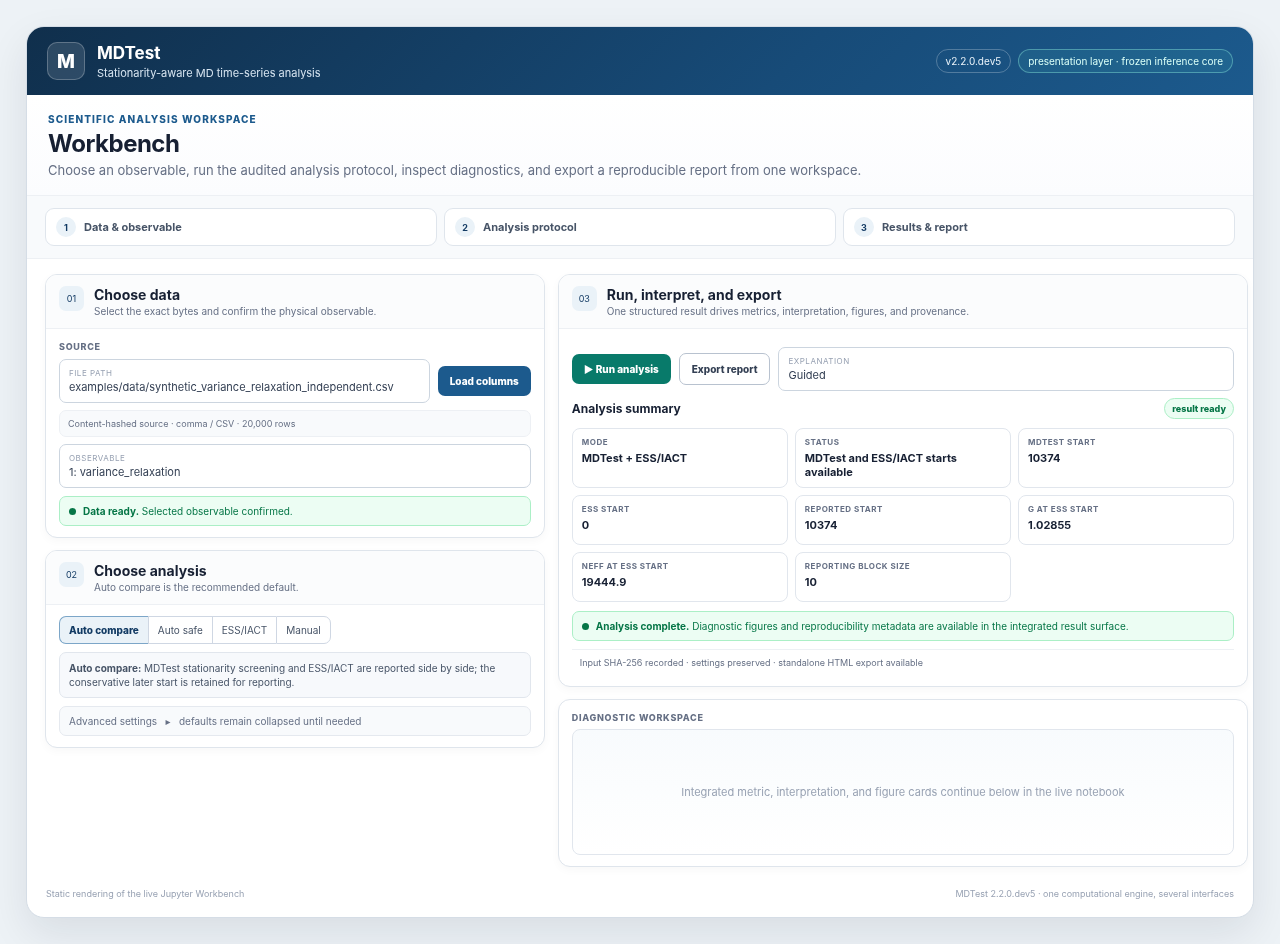
\includegraphics[width=0.98\textwidth]{manual_assets/fig_workbench_overview.png}
\caption{Static rendering of the MDTest Workbench layout.  The distributed notebook provides the live interactive controls; the interface separates data selection, analysis choices, and the result/export stage.}
\end{figure}

\chapter{Python interface}
\section{Auto Safe}
\begin{lstlisting}[language=Python]
import mdtest
r = mdtest.auto_safe(
    "trajectory.csv",
    col=1,
    m_trend_grid=[2,5,10,20,40],
    min_blocks=24,
)
print(r.selected_ts_sw)
print(r.selected_m_corr)
\end{lstlisting}
By default the Python API returns objects and does not write files. Use \texttt{write\_outputs=True} and \texttt{make\_plots=True} when file output is desired.

\section{Auto Compare}
\begin{lstlisting}[language=Python]
r = mdtest.auto_compare(
    "trajectory.csv", col=1,
    write_outputs=True,
    make_plots=True,
    outdir="results/run1",
)
print(r.auto_safe.selected_ts_sw)
print(r.ess.selected_ts_ess)
print(r.selected_ts_star)
\end{lstlisting}

\section{ESS/IACT only}
\begin{lstlisting}[language=Python]
e = mdtest.ess("trajectory.csv", col=1)
print(e.selected_g, e.selected_neff)
\end{lstlisting}

\section{Manual}
\begin{lstlisting}[language=Python]
r = mdtest.manual("trajectory.csv", col=1,
                  ts=600000, m=30, n="max")
\end{lstlisting}

\section{Convenience dispatcher}
\begin{lstlisting}[language=Python]
r = mdtest.analyze("trajectory.csv", mode="auto-safe", col=1)
\end{lstlisting}

\chapter{Command-line and configuration-file use}
\section{Command-line examples}
\begin{lstlisting}[language=bash]
mdtest manual --file trajectory.csv --col 1 --ts 600000 --m 30 --n max

mdtest auto-safe --file trajectory.csv --col 1 \
  --m-trend-grid 2,5,10,20,40 --min-blocks 24

mdtest auto-compare --file trajectory.csv --col 1 \
  --m-trend-grid 2,5,10,20,40
\end{lstlisting}
Use \texttt{mdtest <mode> --help} for mode-specific options.

\section{Configuration files}
Configuration-file mode is intended for recorded, repeatable choices. The first line must be \texttt{MD Test Format}; subsequent lines use key-value entries described in \texttt{docs/CONFIG\_REFERENCE.md}. Unknown keys are rejected rather than silently ignored.

\chapter{Understanding the output}
\section{Trajectory/start plot}
This plot overlays the raw scalar time series with the MDTest stationarity start, ESS start, and final combined start when available. Use it to verify that selected starts make physical sense in the context of visible transients or state changes.

\section{Multi-resolution p-value map}
The two panels show mean-trend and dispersion-trend p-values as functions of candidate start and diagnostic block size. The selected start must satisfy the configured trend criteria across the admissible diagnostic grid. A broad region of passing values is usually more reassuring than an isolated borderline transition.

\begin{figure}[h]
\centering
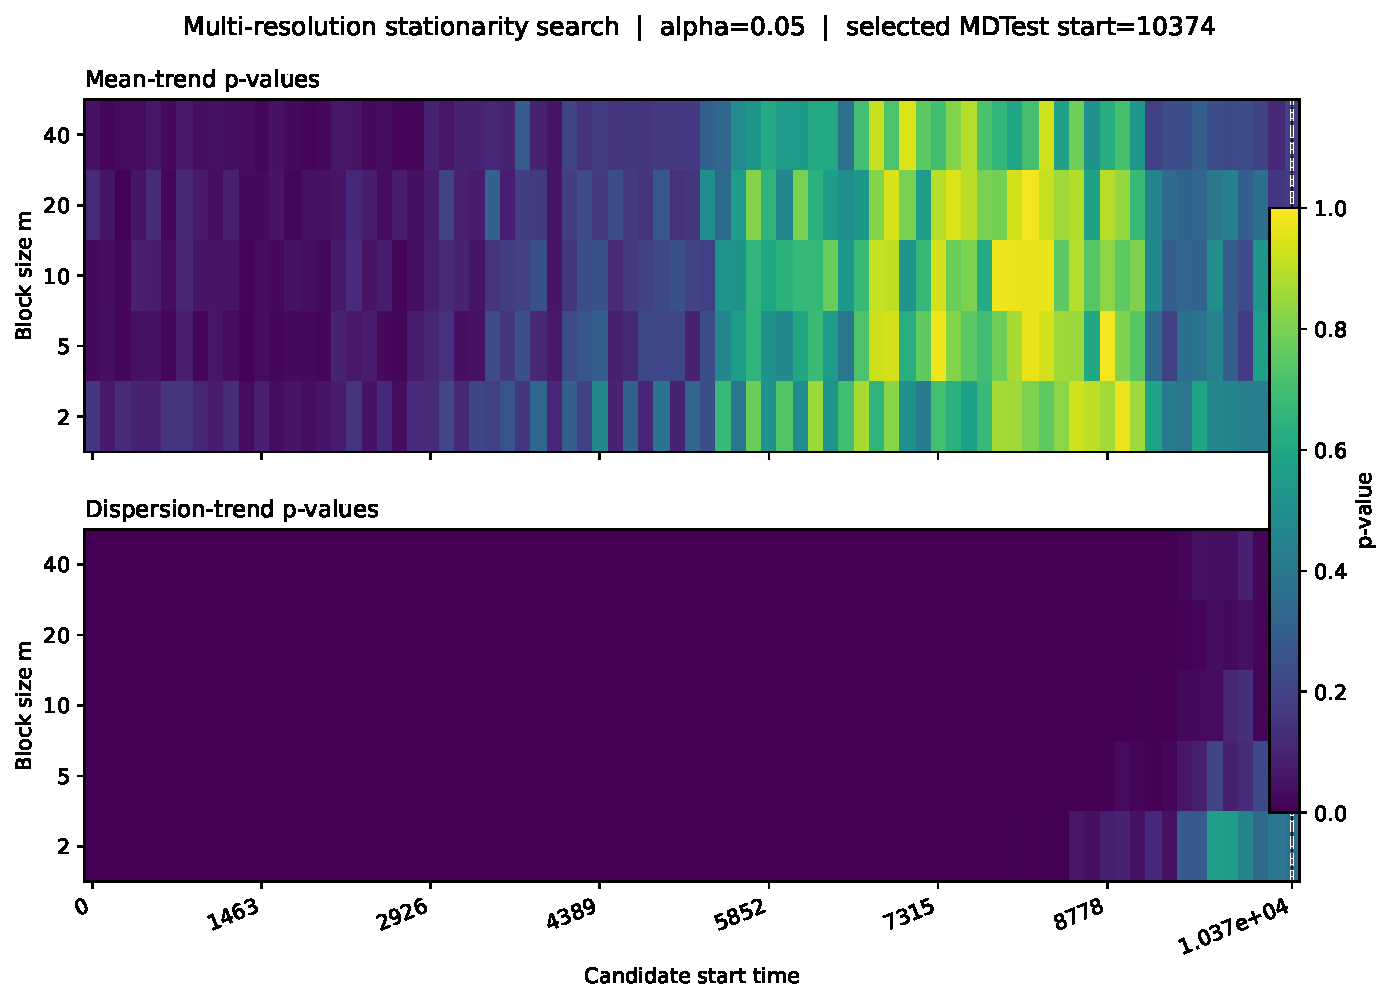
\includegraphics[width=0.98\textwidth]{manual_assets/fig_multiresolution_round3b.pdf}
\caption{Example multi-resolution stationarity map from the released variance-relaxation benchmark.}
\end{figure}

\section{ESS scan}
The ESS scan shows $g$ and/or $N_{\rm eff}$ as the candidate start changes. A large $g$ indicates strong stationary correlation; an early ESS start does not guarantee that mean or variance transients are absent.

\section{Block means}
Inspect the retained block means for slow drift, isolated transitions, oscillatory structure, or too few blocks. The reported horizontal mean line is a statistical summary, not a substitute for the diagnostic pattern.

\section{Four-test summary}
The final panel reports the trend, normality, and residual-correlation checks at the reporting scale. ``Pass'' means no statistically significant violation was detected at the configured significance level; it does not prove the assumption.  Numerical mean, standard-error, or confidence-interval fields can still be computed in some failing cases, but a failed diagnostic means the usual parametric interpretation is not fully supported and should be treated as a warning rather than as a validated production summary.

\chapter{Interpreting common outcomes}
\begin{table}[h]
\centering
\begin{tabularx}{\textwidth}{lYY}
\toprule
Observation & Interpretation & Typical action\\
\midrule
Mean trend fails & retained average is still changing monotonically & move start later; inspect transition\\
Dispersion trend fails & fluctuation magnitude changes with time & move start later; inspect variance/physical transition\\
Shapiro fails & block means do not support normal-theory reporting at this scale & increase $m$, collect more data, bootstrap/nonparametric analysis\\
Von Neumann fails & adjacent block means retain positive persistence & increase $m$ or collect more data\\
SW start much later than ESS start & stationarity screen sees a transient not reflected in ESS efficiency & inspect mean/dispersion maps and trajectory\\
ESS start much later than SW start & retained data may be stationary but strongly correlated & inspect autocorrelation/ESS and use later start if following combined mode\\
No reporting $m$ passes & insufficient length, persistent nonnormality, or strong correlation & longer simulation or different uncertainty method\\
\bottomrule
\end{tabularx}
\end{table}

\chapter{Worked examples}
\section{Independent variance relaxation: Auto Compare}
This released benchmark is independent in time but has a changing fluctuation scale.  It is therefore a useful demonstration of why stationarity assessment and correlation correction answer different questions.  From the root of the unpacked source distribution, run:
\begin{lstlisting}[language=Python]
import mdtest
r = mdtest.auto_compare(
    "examples/data/synthetic_variance_relaxation_independent.csv",
    col=1,
    m_trend_grid=[2, 5, 10, 20, 40],
    m_corr_grid=[10, 20, 40, 80, 160, 320],
)
print(r.auto_safe.selected_start_index_sw)
print(r.ess.selected_start_index_ess)
print(r.selected_start_index_star)
print(r.ess.selected_g)
print(r.auto_safe.selected_m_corr)
\end{lstlisting}
For the released file and frozen algorithm this prints, apart from ordinary floating-point formatting,
\begin{lstlisting}
10374
0
10374
1.0285490983959442
10
\end{lstlisting}
The ESS comparator keeps the complete trajectory because there is essentially no temporal correlation in the mean, whereas the dispersion-trend screen detects the relaxing fluctuation scale and selects the later stationarity start.

\section{Independent mean drift: Auto Safe}
The companion mean-drift benchmark is also independent in time, but its mean relaxes before production.  Run:
\begin{lstlisting}[language=Python]
import mdtest
r = mdtest.auto_safe(
    "examples/data/synthetic_mean_drift_independent.csv",
    col=1,
    m_trend_grid=[2, 5, 10, 20, 40],
    m_corr_grid=[10, 20, 40, 80, 160, 320],
)
print(r.selected_start_index_sw)
print(r.selected_m_corr)
print(r.manual_result.mean)
\end{lstlisting}
The protected manuscript-scale result is
\begin{lstlisting}
9709
10
-0.001293179522305782
\end{lstlisting}
These examples are regression-protected values for the released benchmark files; they are not general thresholds for other trajectories.

\section{NarK volume}
The NarK example illustrates a real correlated MD observable. The multi-resolution search reduces dependence on one initial block length; the ESS comparator reports substantial autocorrelation and may choose a later start. Use the released configuration/example files to reproduce the manuscript tables.  Because the public source distribution contains the example data and configurations whereas an installed wheel need not contain the repository-level example tree, run these reproduction examples from an unpacked source distribution.

\chapter{Troubleshooting}
\section{The file loads but the observable list is wrong}
Check delimiter, header/unit rows, and whether the selected source is the path or upload you intended. Reload columns after changing source or parsing controls.  A file whose name ends in \texttt{.csv} is read as comma-delimited by the frozen loader; use a suitable text extension such as \texttt{.txt} or \texttt{.dat} for whitespace-delimited data, or convert the file to a conventional comma-separated CSV.

\section{Too few blocks}
A candidate start/block size is feasible only when enough complete blocks remain. Reduce $m$, move the start earlier only if scientifically justified, or collect a longer trajectory.

\section{Shapiro--Wilk repeatedly fails}
Remember that the test is on block means. Try larger blocks while keeping enough block samples. For strongly multimodal or long-memory observables, a Gaussian/Student-$t$ summary may simply be inappropriate.

\section{Oscillatory correlations}
The default von Neumann test is one-sided for positive adjacent-block persistence. Strong underdamped oscillation can make both block-level and IACT diagnostics sensitive to scale/truncation. Inspect the raw/autocorrelation pattern and consider larger blocks or a model-based estimator.

\section{Export fails after the input changed}
This is deliberate provenance protection. Restore the analyzed file or rerun MDTest on the current file before exporting raw-data-dependent figures.

\chapter{Validation, reproducibility, and provenance}
The scientific engine is protected by regression tests against manuscript-scale benchmark values. The source distribution includes unit/interface tests, CLI smoke tests, frozen-engine hash checks, and benchmark regeneration scripts. Structured results carry the inference-controlling settings and environment/input provenance. For publication or collaboration, archive the JSON result together with the exact input file and software version.

\chapter{License and citation}
MDTest is distributed under the MIT License. The license permits use, modification, publication, and redistribution of the software and associated documentation, provided the copyright and permission notice are retained in copies or substantial portions. The software is provided without warranty; see the distributed \texttt{LICENSE} file for the controlling text.

The detailed manual is therefore appropriate to distribute inside the software package. The journal manuscript should summarize the program and point readers to the distributed manual rather than reproducing the manual itself.

For scientific use, cite the associated MDTest manuscript and the primary methods relevant to the analysis.

\appendix
\chapter{Default parameters}
\begin{center}
\begin{tabularx}{\textwidth}{l l Y}
\toprule
Quantity & Default & Meaning\\
\midrule
$\alpha$ & 0.05 & diagnostic significance level\\
$n_{\min}$ & 24 & minimum retained blocks for MDTest block diagnostics\\
Trend grid & 2,5,10,20,40 & diagnostic block sizes in automatic stationarity search\\
Reporting grid & 5,10,20,30,40,60,80,120,160,240,320,480 & candidate reporting block sizes\\
ESS minimum lag & 3 & earliest lag after which a non-positive ACF can terminate integration\\
\bottomrule
\end{tabularx}
\end{center}
Defaults are starting points, not universal physical constants. Users should inspect whether block sizes are sensible relative to the dominant time scales of the observable.

\chapter{Package map}
\begin{description}
\item[\texttt{src/mdtest/api.py}] public Python entry points.
\item[\texttt{src/mdtest/analysis.py}] automatic/manual orchestration using the frozen statistical primitives.
\item[\texttt{src/mdtest/diagnostics.py}] block construction and four-test primitives.
\item[\texttt{src/mdtest/autocorrelation.py}] FFT autocorrelation, statistical inefficiency, ESS-start scan.
\item[\texttt{src/mdtest/results.py}] structured result/settings/provenance dataclasses.
\item[\texttt{src/mdtest/workbench.py}] Jupyter Workbench controller and widgets; no duplicate statistical engine.
\item[\texttt{src/mdtest/visualization.py}] Workbench diagnostic figures.
\item[\texttt{src/mdtest/presentation.py}] guided/technical text and HTML/report export.
\item[\texttt{docs/}] architecture, API, configuration, Workbench, scientific-freeze, and audit documentation.
\item[\texttt{examples/}] released data, configurations, and Workbench demonstration.
\item[\texttt{testingScripts/}] scientific regression and packaging checks.
\end{description}

\begin{thebibliography}{99}
\bibitem{SchiferlWallace1985} S.K. Schiferl and D.C. Wallace, Statistical errors in molecular dynamics averages, J. Chem. Phys. 83 (1985) 5203--5209.
\bibitem{Mann1945} H.B. Mann, Nonparametric tests against trend, Econometrica 13 (1945) 245--259.
\bibitem{Kendall1975} M.G. Kendall, Rank Correlation Methods, 4th ed., Charles Griffin, London, 1975.
\bibitem{ShapiroWilk1965} S.S. Shapiro and M.B. Wilk, An analysis of variance test for normality (complete samples), Biometrika 52 (1965) 591--611.
\bibitem{Fenwick1994} P.M. Fenwick, A new data structure for cumulative frequency tables, Software: Practice and Experience 24 (1994) 327--336. doi:10.1002/spe.4380240306.
\bibitem{KleinbergTardos2006} J. Kleinberg and E. Tardos, Algorithm Design, Addison-Wesley, 2006 (merge-sort inversion counting as a related textbook technique).
\bibitem{Flyvbjerg1989} H. Flyvbjerg and H.G. Petersen, Error estimates on averages of correlated data, J. Chem. Phys. 91 (1989) 461--466.
\bibitem{Chodera2016} J.D. Chodera, A simple method for automated equilibration detection in molecular simulations, J. Chem. Theory Comput. 12 (2016) 1799--1805.
\end{thebibliography}

\end{document}
